%\documentclass[varwidth,border=10pt]{standalone}
\documentclass[aps,pra,twocolumn,superscriptaddress]{revtex4-1} %reprint
\thispagestyle{empty}
%\usepackage{subcaption}
%\usepackage[labelformat=parens,labelsep=quad, skip=3pt]{caption}
\usepackage{etex}
\usepackage{amsmath}
\usepackage{bm}
\usepackage{bbm}
\usepackage{listings}
% % \textwidth 16cm \textheight 23.5cm
% \renewcommand{\baselinestretch}{1.2}
\usepackage{graphicx}
\usepackage{graphics}
\usepackage{epsfig}
\usepackage{color}
\usepackage[dvipsnames]{xcolor}
\usepackage{multirow}
\usepackage[colorlinks]{hyperref}
\usepackage{fancyhdr}
\usepackage{calc}
\usepackage{natbib} %[numbers]
\usepackage{bibentry}
\usepackage{bbm}
\usepackage{bbold}

% todo list and commands
%\usepackage{todonotes}
%% to avoid the conflict with amths package % not working
%\makeatletter
%\providecommand\@dotsep{5}
%\makeatother
%\listoftodos\relax
%\usepackage{makeidx}
%\allowdisplaybreaks
%% for eps transfering to pdf.
%\usepackage[update,prepend]{epstopdf}
%\usepackage{ifpdf}
%
%\ifpdf
%   \usepackage{graphicx}
%   \usepackage{epstopdf}
%   \epstopdfsetup{suffix=}
%   \DeclareGraphicsRule{.eps}{pdf}{.pdf}{`epstopdf #1}
%   \pdfcompresslevel=9
%\else
%   \usepackage{graphicx}
%\fi
% subfig
\usepackage{mwe}
\usepackage[caption=false]{subfig}
% to fix a figure's position using [H] option of thec figure.
\usepackage{float}
% to use \lesssim and other math symbols
%\usepackage{amssymb}
% set package options
\captionsetup[subfloat]{position=top,singlelinecheck=off,labelfont={normalsize,sf}, %justification=raggedright,
  labelformat=simple,listofformat=subparens,aboveskip=0pt,parskip=0pt,farskip=5pt,
  captionskip=0pt}

% customize subfigure label to capitals
\renewcommand{\thesubfigure}{(\alph{subfigure})}
  
  %==== scattering and optical pumping rates ====%
  \newcommand{\gammauu}{\gamma_{\uparrow \rightarrow \uparrow}}
  \newcommand{\gammadd}{\gamma_{\downarrow \rightarrow \downarrow}}
  \newcommand{\gammaud}{\gamma_{\uparrow \rightarrow \downarrow}}
  \newcommand{\gammadu}{\gamma_{\downarrow \rightarrow \uparrow}}
  \newcommand{\gammau}{\gamma_{\uparrow}}
  \newcommand{\gammad}{\gamma_{\downarrow}}
  
  %==== effective areas ======
  \newcommand{\Ain}{A_{\rm in}}
  \newcommand{\Abir}{A_N}
  \newcommand{\AF}{A_{\rm Far}} % for the Faraday protocol.
  \newcommand{\Ai}{A_{\rm in}} % for the input light.
  \newcommand{\Aint}{A_{\rm int}} % for the interaction area.
  
\begin{document}
\begin{figure}[htb]
\centering
 \begin{minipage}[h]{0.27\linewidth}
 %\begin{tabular}{*{2}{b{0.2\textwidth-2\tabcolsep}}}
  \subfloat[h][$1/\AF$]{
    %\input{fig/square waveguide_invA_Far_xy.tex}
    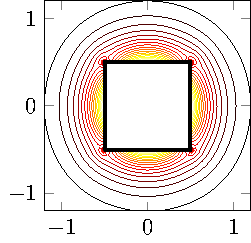
\includegraphics[width=\linewidth]{../Fig4a}
    }
    \hfill
  \subfloat[h][$ 1/\Ain $]{
      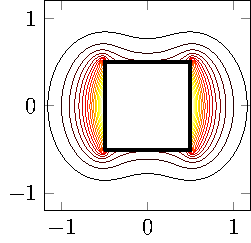
\includegraphics[width=\linewidth]{../Fig4b}
      %\input{fig/square waveguide_invA_in_xy.tex}
      }
   \end{minipage}\hfill
   \begin{minipage}[h]{0.73\linewidth}
   \vspace{-9pt}
   \subfloat[h][$ C_1 $]{
      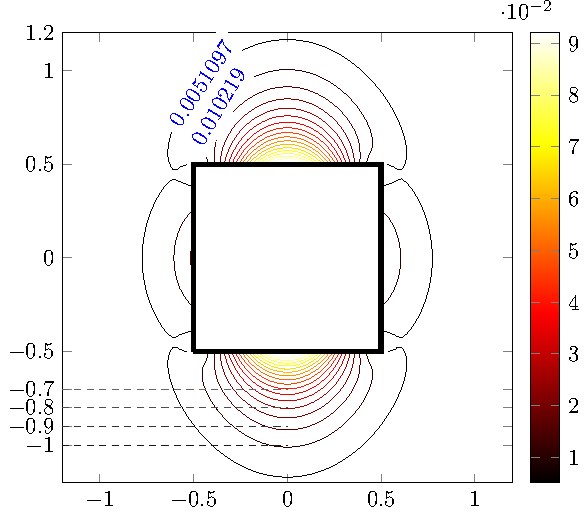
\includegraphics[width=\linewidth]{../Fig4c}
      %\input{fig/square waveguide_C1_xy.tex}
      }
   \end{minipage}
\end{figure}
\end{document}